\documentclass[a4paper,10pt]{article}
%In the preamble section include the arabtex and utf8 packages
\usepackage{arabtex}
\usepackage{utf8}
\usepackage{url,graphicx}

%remove ugly boxes from pdf-embedded links.
\usepackage{hyperref,xcolor}
\hypersetup{%
      colorlinks=false,% hyperlinks will be black
            linkbordercolor=black,% hyperlink borders will be red
              pdfborderstyle={/S/U/W 0}% border style will be underline of width 1pt
}

\begin{document}
%start encoding to unicode
%Note that your layout must support arabic text when compiling
\setcode{utf8}




\title{Proposal to Add Emoji Symbol for {\sc Falafel} to Unicode}
\author{Ben Klemens with Emojination\\ {\tt ben@klemens.org}}
\date{4 April 2018 Revision}
\maketitle

\begin{abstract}
This proposal requests the addition of a {\sc falafel} emoji to a future version of the
Unicode standard.  The emoji food set is lacking in Middle Eastern and North African
foods, and in unambiguously vegetarian, kosher, or halal foods outside of fruits and
vegetables. A falafel emoji addresses these gaps.
\end{abstract}


\section{Introduction, Identification, Images}

{\sc Falafel} is a ball of fried chickpeas or fava beans, and is popular in the Middle East
and North Africa, and increasingly throughout the world.  One of its key advantages is
that it accommodates a range of food preferences: given reasonable care in preparation,
it is vegan and vegetarian, halal, and kosher (for the remainder of this proposal, ``VHK'')

\begin{figure}[h]
\begin{center}
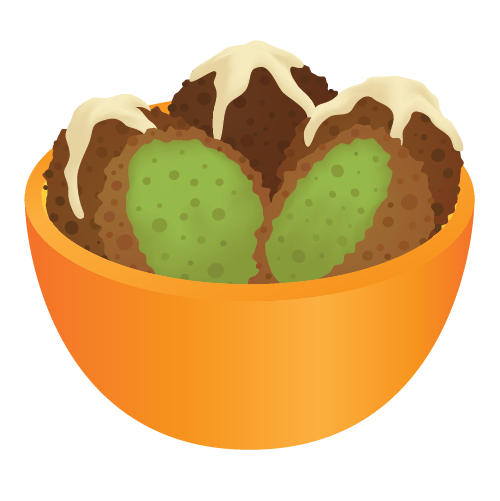
\includegraphics[width=2.2in]{falafel-bowl-tahini.png}
\end{center}
\caption{Sample emoji renderings by Aphee Messer, in a bowl and with common toppings.}
\label{apheefig}
\end{figure}

\begin{figure}[h]
\begin{center}
\begin{tabular}{cc}
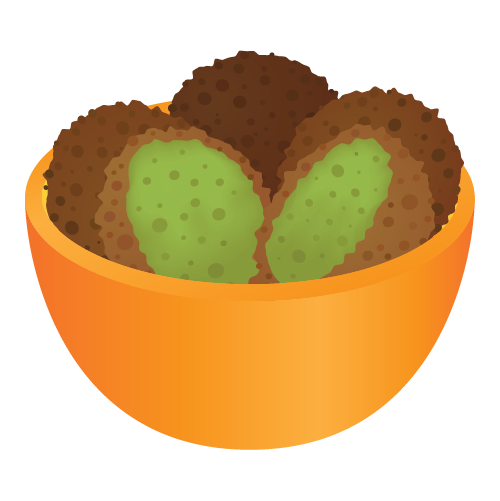
\includegraphics[width=2.2in]{falafel-bowl.png}& 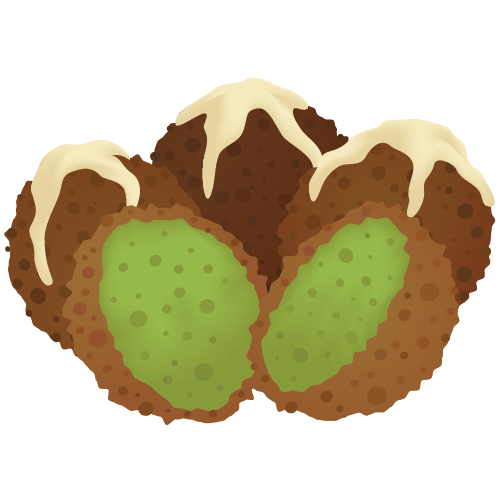
\includegraphics[width=2.2in]{falafel-tahini.png}
\end{tabular}
\end{center}
\caption{Additional renderings by Aphee Messer.}
\label{apheefigtwo}
\end{figure}

Falafel is often topped with hommous, tahini,
or babaganouj, which conveniently all have a similar sandy color. 
The proposed emoji would picture a few falafel balls in a bowl, covered with one of these
toppings, with one split open to reveal the green interior of the ball.  
Figure \ref{apheefig} presents
a sample rendering. 
To aid in visualizing alternatives, the left illustration
of Figure \ref{apheefigtwo} shows balls of falafel in a bowl without any topping, and the right
illustration shows toppings without a bowl.

The food category in the emoji set includes a wide range of fruits and vegetables, but
very little else that is VHK. For example, cheeses may not be VHK due to rennet, and the
Japanese origins of emoji have led to a wide range of explicitly or likely
shellfish-based food emoji. The current emoji set has good representation of foods
from the American and East Asian regions, but very little from the Middle East and
North Africa.


Made with chickpeas, the dish is always {\em falafel}, but made with fava beans, the dish
is sometimes named {\em falafel} and sometimes {\em ta'amia} (\<طعمية>), depending upon the
region or the whims of the chef. Search results gauging the popularity of {\sc ta'amia} give
ambiguous results, but it is suggested as an alternative name for the proposed emoji.

\section{Expected Usage}

Because the {\sc falafel} emoji is intended to address under-representation of VHK foods in the
emoji food set, it is worth noting that
the world's VHK population is substantial. The Indian Census estimates that
in 2014, 28.4\% of Indian men and 29.3\% of Indian women were
vegetarian.\footnote{Registrar General and Census Commissioner
of India, ``Sample Registration System Baseline Survey 2014''.
\url{http://www.censusindia.gov.in/vital_statistics/BASELINE\%20TABLES07062016.pdf}}
With 1.27 billion Indians in 2014, this gives circa 366 million vegetarians.
Our rough calculations using a large-scale worldwide survey by the Pew Forum gives an estimate
of 796 million Muslims likely to be halal,\footnote{
Estimate by the authors primarily based on a Pew Forum survey
of 38,000 Muslims in 39 countries.  See {\em The World's
Muslims: Religion, Politics and Society}, by Lugo, Cooperman, et al.  at
\url{http://assets.pewresearch.org/wp-content/uploads/sites/11/2013/04/worlds-muslims-religion-politics-society-full-report.pdf}.
Full details on the calculation are given in the repository supporting this document,
at \url{https://github.com/b-k/unicode-falafel}.
} which already gives just over 1.1 billion VHK eaters,
without even counting vegetarians outside India, Muslims outside the Pew study area, or
kosher eaters.


\subsection{Frequency}\label{freqsec}


\begin{figure}
\begin{center}
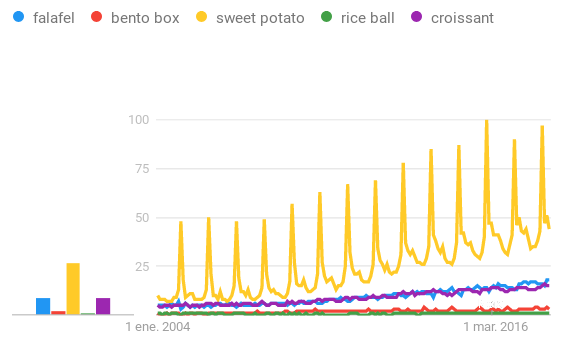
\includegraphics[width=3.5in]{trends.png}
\end{center}
\caption{In English, ``Falafel'' is as common as ``croissant'' in Google's database.}
\label{engplot}
\end{figure}


Figure \ref{engplot} shows frequencies of various food terms in Google's English-language
database of user searches.  In this data set, the usage of ``falafel'' is roughly as popular as
``croissant.'' 
The figure includes ``sweet potato,'' which is more popular
in Google's database but clearly seasonal, while falafel shows consistent usage.
Some of the emoji related to Japanese food, {\sc rice ball} and {\sc bento box}, are also
presented for comparison, though they may not be ideal for comparison to falafel.

To preserve the scale, ``rice'' was omitted from the plot of English search terms:
being a basic staple, it was searched on Google 17 times more often than ``falafel.''

\begin{figure}
\begin{center}
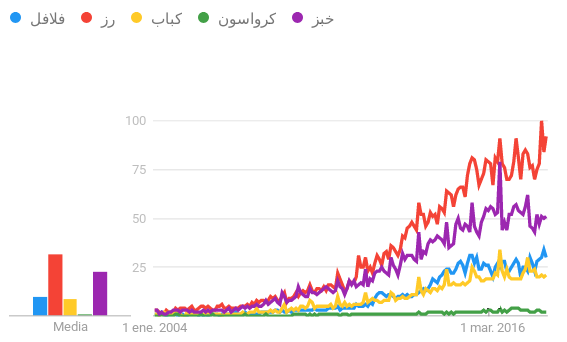
\includegraphics[width=3.5in]{atrends.png}
\end{center}
\caption{In Arabic, ``Falafel'' competes with basic staples in search popularity.}
\label{aplot}
\end{figure}

But among Arabic search terms, falafel is in the same range as basic staples. 
Figure \ref{aplot} shows search frequencies in Google's database in Arabic.
``Rice'' (\<رز>, in red) appears in the database of searches only three times as often as
falafel (\<فلافل>, in blue).  Another staple, ``bread'' (\<خبز>, in purple) is only 70\% more
popular than falafel at the end of this period. Falafel seems slightly more popular than ``kebab'' (\<كباب>,
in yellow), while ``croissant'' (\<كرواسون>, in green) seems largely unknown.\footnote{
Ta'amia is largely unknown in English, with only 469,000 hits in Google and 14,000 in Bing.
Its search behavior is anomalous in Arabic search engines: Bing gives 53,000 hits compared
to 301,000 for falafel (17.6\%), and Youtube gives 26,200 hits compared to 460,000 for falafel (5.7\%), but
Arabic Google gives 4.9 million hits, not far behind the 5.67 million hits for falafel.
Counts from boolean searches can be unreliable, but searching Google for pages that mention ta'amia but not falafel
(``\<طعمية> -\<فلافل>'')
returns 4.3 million hits, while Google counts 4.1 million pages mentioning falafel but not ta'amia
(``\<فلافل> -\<طعمية>''), for a total of 8.4 million pages, not far behind the count for rice.
Because of these ambiguous results, ta'amia is omitted from the tables of results.
}

Trends in image searches are presented in the appendix in Figures \ref{engpicplot} and \ref{apicplot}.
The results are largely similar, but rice is somewhat more common in Arabic image searches
and English speakers are enamored of croissant photos.


\begin{figure}
\hspace{-2cm}
\begin{tabular}{rr}

\begin{tabular}{l|rrr}
{\bf English, count} & Bing & Google & YouTube \\\hline
Falafel  & 6,460 & 25,000 & 301\\
Rice    & 21,900 & 607,000 & 13,500\\
Sweet potato & 13,700 & 46,200 & 786\\
Croissant & 12,100 & 91,800 & 537 \\
Bento box & 2,160 & 8,760 & 229 \\
Rice ball & 926 & 1,010 & 154\\
\end{tabular}

&

\begin{tabular}{l|rrr}
{\bf English, scaled} & Bing & Google & YouTube \\\hline

Falafel  &1.00& 1.00 & 1.00 \\
Rice    &3.39&24.28 & 44.85 \\
Sweet potato &2.12& 1.85 & 2.61 \\
Croissant &1.87& 3.67 & 1.78 \\
Bento box &0.33& 0.35 & 0.76 \\
Rice ball &0.14& 0.04 & 0.51
\end{tabular}
\\
\phantom{Filler}\\

%Couldn't get Arabic working in tables...
\begin{tabular}{l|rrr}
{\bf Arabic, count} & Bing & Google & YouTube \\\hline
%\<ﻑﻼﻔﻟ>
Falafel & 301  & 5,670 & 460\\
%\<ﺃﺭﺯ>
Rice & 1,690& 10,400 & 595\\
%\<ﺦﺑﺯ>
Bread  & 601& 72,200   & 703\\
%\<ﻚﺑﺎﺑ>
Kebab & 303 & 2,650   & 625\\
%\<ﻙﺭﻭﺎﺳﻮﻧ>
Croissant & 62.2 & 405 & 63.7
\end{tabular}

&
\begin{tabular}{l|rrr}
{\bf Arabic, scaled} & Bing & Google & YouTube \\\hline
Falafel & 1.00 & 1.00  & 	1.00\\
Rice & 5.61 & 1.83	 &  1.29\\
Bread & 2.00 & 12.73 &    1.53\\
Kebab & 1.01 & 0.47	 &  1.36\\
Croissant & 0.21 & 0.07	 &  0.14
\end{tabular}

\end{tabular}
\caption{Search engine hits in thousands, from three search engines. Counts are given on
the left, and as a percent of the falafel count to the right.}
\label{counttab}

\end{figure}

Figure \ref{counttab} shows the search result counts in three search engines, in English
and Arabic. Apart from Arabic Google's anomalous count for bread, the results largely
follow those from the trend lines: in English, falafel result counts are behind but
on the same order of magnitude as sweet potatoes and croissants, while in Arabic, the
falafel result counts are behind but on the same order of magnitude as rice and bread.


\subsection{Use in sequences}\label{seqsec}
{\sc falafel} as street food is served as a wrap or in a flatbread, so sequencing it before {\sc stuffed flatbread}
facilitates the {\sc falafel}
+ {\sc stuffed flatbread} pairs, which could transform the wrap and flatbread emoji
into unambiguous representations of a falafel wrap or pita. {\sc falafel} + {\sc salad} is
another common menu item. Some Western restaurants serve a falafel burger as a vegetarian option,
which users might represent via {\sc falafel} + {\sc hamburger}.


\subsection{Image distinctiveness}
The ideal falafel is briefly fried so that the exterior is brown, but the interior
remains green, which is a relatively distinctive appearance. Other brown balls with
a green interior, such as some fruit, are unlikely to be arranged in a bowl or covered
in a sauce. The brown-to-green pattern is distinctive and easily recognized even in
small fonts. However, we leave it to the vendors to choose the most effective designs.

\subsection{Completeness}
Falafel would be the first VHK Middle Eastern food represented in emoji.
Middle Eastern food has almost no representation in emoji. For various reasons, distinctive foods
commonly found in the melting pot of Middle Eastern cuisine such as tahini, shakshuka or
baklava are missing. 
{\sc Hummus} has been previously proposed and rejected by the Unicode Technical Committee. 
 D\"oner kebab has an emoji in the form
of {\sc stuffed flatbread}. The proposal itself, ``UTC document
L2/15-084,''\footnote{\url{http://www.unicode.org/L2/L2015/15084-kebab.pdf}} makes
only brief reference to its Turkish origins and instead bills it as ``Germany's most
favorite fast food snack;'' the final emoji is further generalized to cover cuisines from around the world.

\section{Selection Factors for Exclusion}

\subsection{Overly specific}

{\sc Falafel} has a level of specificity comparable to many other emoji, such as
{\sc croissant}, {\sc broccoli}, or {\sc sweet potato}.
%And it is as prominent for a particular
%region of the world which is currently underrepresented.

\subsection{Open ended}

Falafel recipes are largely uniform, so there is no need for additional emoji for
different falafel subtypes. One can find recipes for flatter discs or donut-shaped
falafel, but we believe these are relatively uncommon and the traditional ball is
sufficient to express the idea of falafel. The proposed image is a reasonable
representation of the fava-based dish, be it named {\em falafel} or {\em ta'amia}.
% In addition, in our quick unscientific poll of Middle
%Easterners, falafel ranks among the highest for both being culturally relevant, and
%visually distinctive. In contrast, 
The universe of iconic and visually distinctive foods in the Middle East is fairly scoped.

\subsection{Already Representable}

``Emoji Additions Tranche 6: More Popular Requests
and Gap Filling''\footnote{UTC document L2/15 195R2,
\url{https://www.unicode.org/L2/L2015/15195r2-emoji-add-tranche6.pdf}} does propose
``falafel'' as an alias, but the image is deliberately ambiguous. The proposal describes
``frybread, pita, [or] focaccia'' stuffed with ``ingredients, such as meat, vegetables,
and condiments,'' and the proposed character in the proposal document shows brown strips that
can not be falafel.  As above, a key feature of falafel is that it is unambiguously VHK.
A VHK eater who answers the question {\em what would you like for dinner?} with {\sc
stuffed flatbread} has no idea what he or she will get.

Falafel is not married to pita. As street food, it is often served in lafah,
a thin wrap producing a dish with closer resemblance to a burrito than a
stuffed pita. One may also find falafel on a mezze plate along with other small
dishes. Expressing the latter use with existing emoji, for example via {\sc stuffed
flatbread + fork and knife with plate}, may leave significant ambiguity that the author
is writing about flatbread containing primarily falafel, minus the flatbread.

\subsection{Transient}

The plot above from Google's database shows consistent usage of ``falafel'' 
since 2004. Pre-Internet, falafel is old enough that its
origins have been lost. Consensus seems to be that ta'amia came first, with falafel an
eventual variant, though it is unknown when the substitution from fava to chick peas
was first made.  Ta'amia may have originated among Christian Copts of Alexandria in
centuries past, or even the times of the pharaohs.

\subsection{Other exclusion factors}
The {\sc falafel} emoji is not a logo, brand, or other excluded category. Although
universally hailed as delicious, we could find no sources that regard falafel as a deity.

Section \ref{freqsec} compared falafel's popularity to that of foods represented by early
emoji such as bento boxes and rice balls, but these comparisons are only one part of the
overall range, and the argument does not hinge on those comparisons.

No exact image is required.

\section{Location on the emoji keyboard}

As per Section \ref{seqsec}, falafel is well-paired with wraps and flatbreads, so 
sequencing it before {\sc stuffed flatbread}
facilitates the {\sc falafel} + {\sc stuffed flatbread} pairs.

\vfill
{\small \paragraph{About}
This proposal has a supporting repository of documents at 
\url{https://github.com/b-k/unicode-falafel}.

This document owes a debt Jennifer 8. Lee for editing and extensive
advice, Ronit Klemens for her expertise in Middle Eastern cuisine,
and Aphee Messer for her visualizations.

Ben Klemens is an economist who has worked heavily in tech and software policy issues,
including at the Brookings Institution and the Free Software Foundation. He tries to
be a diverse eater, so only about 15\% of his diet is falafel.
}

\eject
\section*{Appendix}
The specifications for emoji proposals require screen shots of searches in several
search engines, and plots Google Trends counts for images. These are provided here
for reference. The counts in Figures \ref{enproof} and \ref{arproof} are transcribed
to Table \ref{counttab}. As per the specification, these searches were done
in a browser's privacy mode. The word {\em falafel} is fairly unique and unambiguously
refers to a food, so the searches were done without additional context (like {\em
falafel food} or {\em falafel dish}).


\begin{figure}[!hb]
\begin{center}
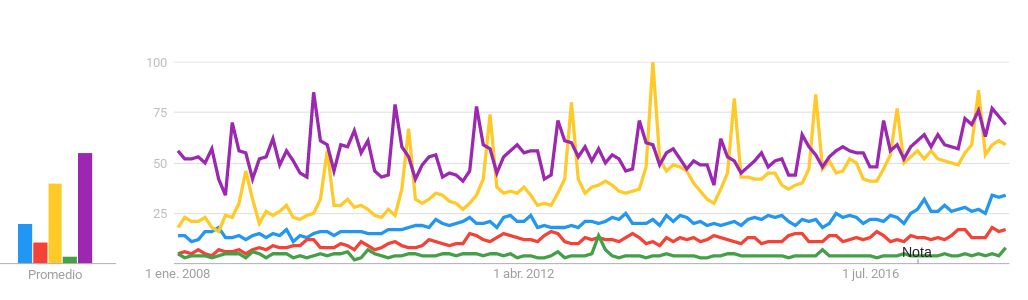
\includegraphics[width=4.8in]{etrends-pics.png}
\end{center}
\caption{Counts of pictures in Google's English database, using the same color key as
Figure \ref{engplot}. Notably, falafel is in blue. Croissants, in purple, are very photogenic.}
\label{engpicplot}
\end{figure}


\begin{figure}[!hb]
\begin{center}
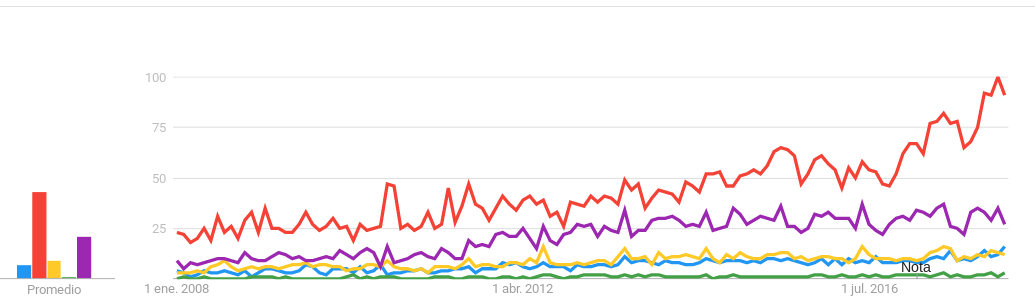
\includegraphics[width=4.8in]{atrends-pics.png}
\end{center}
\caption{Counts of pictures in Google's Arabic database, using the same color key as Figure \ref{aplot}. Rice (red) appears more often than in
the text search result count; falafel (blue) less often, but still commensurate with kebabs (yellow) and not far behind bread (purple).}
\label{apicplot}
\end{figure}

\def\ss#1#2#3{\includegraphics[width=#3]{search_shots/#1-#2.png}}
\def\row#1#2{#1&\ss{b}{#2}{2.5cm}& \ss{g}{#2}{3.4cm}& \ss{y}{#2}{4.5cm}\\\hline}

\begin{figure}
\begin{center}
\begin{tabular}{l|c|c|c|}
 & Bing & Google &YouTube\\
\hline
\row{Falafel}{falafel}
\row{Rice}{rice}
\row{Sweet potato}{sweet_potato}
\row{Croissant}{croissant}
\row{Bento box}{bento_box}
\row{Rice ball}{rice_ball}
\end{tabular}
\end{center}
\caption{Screen shots of English language searches}
\label{enproof}
\end{figure}

\def\ss#1#2#3{\includegraphics[width=#3]{search_shots/#1-#2.png}}
\def\arow#1#2{#1&\ss{b-a}{#2}{2.5cm}& \ss{g-a}{#2}{3.4cm}& \ss{y-a}{#2}{4.5cm}\\\hline}

\begin{figure}
\begin{center}
\begin{tabular}{l|c|c|c|}
 & Bing & Google &YouTube\\
\hline
%\<ﻑﻼﻔﻟ> 
\arow{Falafel}{falafel}
%\<ﺃﺭﺯ>
\arow{Rice}{rice}
%\<ﺦﺑﺯ> 
\arow{Bread}{bread}
%\<ﻚﺑﺎﺑ> 
\arow{Kebab}{kebab}
%\<ﻙﺭﻭﺎﺳﻮﻧ> 
\arow{Croissant}{croissant}
\end{tabular}
\end{center}
\caption{Screen shots of Arabic language searches}
\label{arproof}
\end{figure}

\end{document}
